%
% Capítulo 5
%
\chapter{Frontend Implementation} \label{cap:frontend_implementation}

The frontend application is tasked with data visualization and user interaction. The objective is for the application to provide an intuitive interface for the various users to be able to fulfill the set use cases outlined in section ~\ref{sec:use_cases}.

The frontend is implemented in Typescript and React, and makes use of JSON-Rules-Engine to enforce the form's rules.

A simplified overview of the component interaction and organization is presented in figure \ref{fig:frontend_implementation}.

\begin{figure}[h]
	\begin{center}
		\resizebox{60mm}{!}{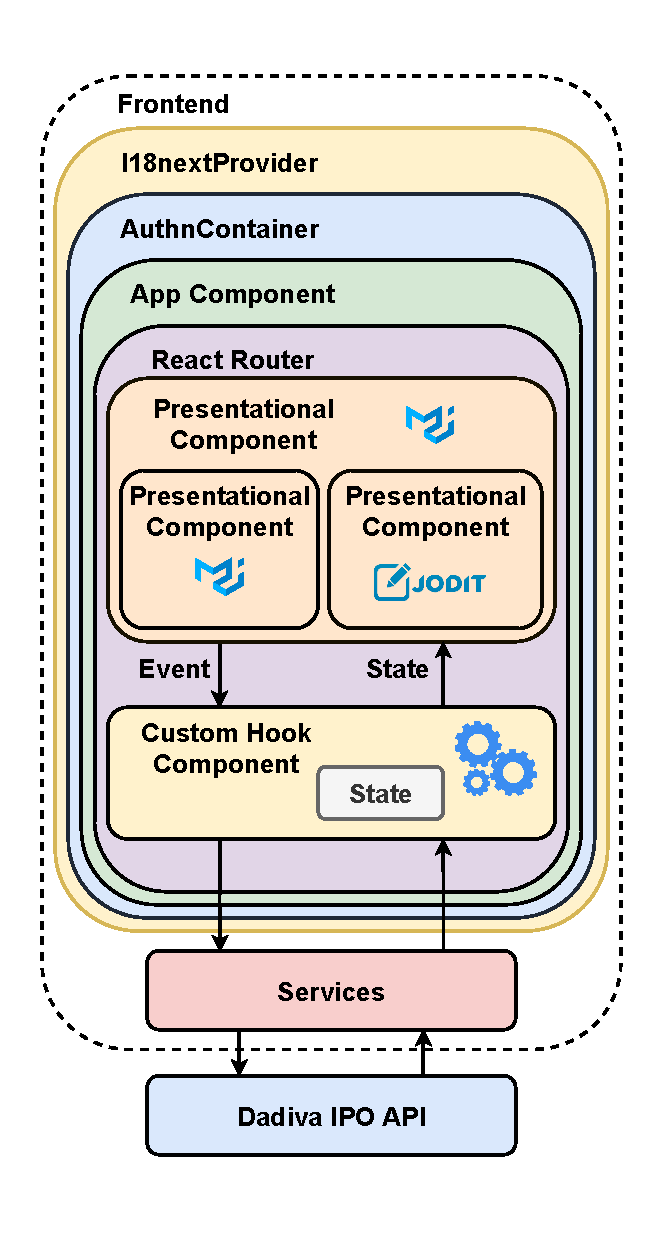
\includegraphics{./figures/frontend_implementation.pdf}}
	\end{center}
	\caption{Simplified Component interaction and organization.}\label{fig:frontend_implementation}
\end{figure}

\newpage

\section{Structure}

The frontend structure is as follows:

\begin{itemize}
	\item src: contains the source code of the application;
	\item public: contains the static files of the application;
	\item package.json:  contains the dependencies of the application;
	\item tsconfig.json: contains the TypeScript configuration;
	\item webpack.config.js:  contains the Webpack configuration.
\end{itemize}

The src folder is then subdivided into multiple folders/files, each being responsible for a different functionality of the application:

\begin{itemize}
	\item components: contains the components of the pages;
	\item domain: contains the domain objects;
	\item pages:  contains the application's pages, each containing various components;
	\item services: contains the services that communicate with the backend application;
	\item session: contains the code needed to maintain a user session.
	\item utils:  contains general utility functions.
\end{itemize}

It should be noted that, folders within the components folder may contain further utils, containing utility functions that are specially pertinent for that component and shouldn't necessarily be in the general utils. 

Furthermore, besides the aforementioned folders, the src folder also contains an index.tsx and App.tsx files. The index.tsx file is the entry point for the application meanwhile the App.tsx is the main component of the React application.


\section{Services}

The frontend services are responsible for communicating with the backend application and, as such, each frontend service as a backend counterpart.

To facilitate this communication we used the Fetch API \cite{Fetch_API}, which enables asynchronous resource requests by returning a promise that resolves to a response for that request.

To expedite, and reduce the code for, the api resource requests we created a fetchAPI function that accepts the request parameters and return a promise that will resolve to the requests response, this function can also handle errors if the response's status code isn't in the 200 family.

To further abstract the api calls,  the fetchAPI function was encapsulated within functions that represent specific HTTP methods, such as GET, POST, PUT and DELETE.

\newpage

\section{Components}

A simplified view of the component tree is presented in Figure ~\ref{fig:reactComponentTree}.
In this chapter we'll mainly focus on the:
\begin{itemize}
	\item \textbf{I18nextProvider}: manages the language preferences of the user;
	\item \textbf{AuthnContainer}: manages the session information;
	\item \textbf{FormPage \& useNewForm}:used to display form to the donor and manage it's state using JSON-Rules-Engine;
	\item \textbf{EditFormPage \& useEditFormPage}:  displays form in the backoffice, to the administrators, and allows to perform change's to the structure, also manage it's state;
	\item \textbf{Editor}: used to display the terms to the administrators and allows to change them. 
\end{itemize}

\begin{figure}[h]
	\begin{center}
		\resizebox{130mm}{!}{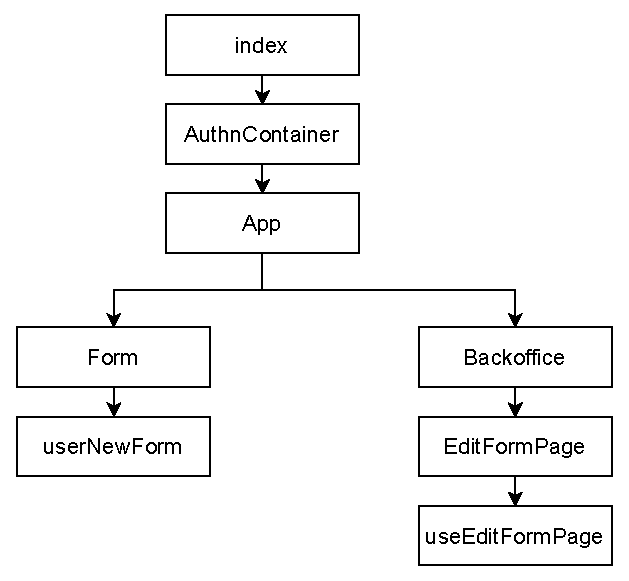
\includegraphics{./figures/reactComponentTree.pdf}}
	\end{center}
	\caption{Simplified React Component Tree.}\label{fig:reactComponentTree}
\end{figure}

\subsection{I18nextProvider}

The I18nextProvider component is part of the i18next library ecosystem, which is used for internationalization (i18n) in JavaScript applications. The purpose of the I18nextProvider component is to integrate i18next into React applications by providing the i18n instance to the component tree.

By accessing the i18n instance, we can set the desired language for the application. This is useful for both the frontend and to request certain resources from the backend, i.e. requesting the resource with the user's language preferences, or default to a certain resource if that isn't available.


\subsection{AuthnContainer}
The AuthnContainer component plays a crucial role in enabling user authentication and consequent storage of the authentication information within the application state.

To do so it uses the React Context API \cite{React_Context_API}, which allows to pass data trough the component tree without having to pass props down manually at every level, thus enabling seamless data sharing between components.

The Session type describe a user's session, i.e. their name and nic. The SessionManager type acts as a wrapper, containing both the session and the methods to manage it, i.e. set a session and delete it.

The AuthContainer component wraps it's child components within it's LoggedInContext.Provider, providing the session manager instance and it's methods as the context value, making the authentication information available throughout the component tree.

\newpage
\subsection{FormPage \& useNewForm}\label{form_implementation}

The concepts in this section build upon those discussed in Section \ref{arc_jre}. It is advised to refer to that section for a thorough understanding.

The FormPage is responsible for form display to donor users. It leverages the useNewForm hook.

The useNewForm hook is a custom React hook designed to manage the state and logic of the form within the frontend application. This hook integrates several important functionalities, including handling form data, managing user interactions, and executing business rules, making it a critical part of the form-handling process.

To do this the hook makes use of the JSON-Rules-Engine. After the form is fetched using the frontend service layer the initial state of the engine is set, an illustration of the following example is presented in Figure \ref{fig:form_implementation}.
Firstly the facts, i.e. the answers, are added to the engine, which state that all the questions haven't been answered, and secondly the rules, which contain the navigation and display logic.

To make sure all questions that should show by default are visible the form has a rule, per question, in which the top level condition, no matter the type, is empty with an event of type showQuestion and referring to the question that should be visible by default, as illustrated in Listing \ref{default_question}.
Once the engine is run, these conditions are met and the respective events are returned.

\begin{lstlisting}[style=sharpc, caption={Condition for visible by default questions}, label={default_question}]
conditions: {
	any: [],
},
event: {
	type: 'showQuestion',
	params: {
		id: 'visibleByDefault'
	},
}
\end{lstlisting}

The hook's states are then updated, mainly, the showQuestions, canGoNext, canGoReview and formAnswers. The showQuestions state stores the questions that are being displayed. The canGoNext state stores if the next group should be available,  by default false when initializing. The canGoReview state stores if all questions where answered and the form can be reviewed, by default false when initializing. The formAnswers state stores all the answers given at any point.
As the user answers the form's questions the formAnswers state is updated and is fed to the engine, which runs again, returning the relevant events.

\begin{figure}[h]
	\begin{center}
		\resizebox{150mm}{!}{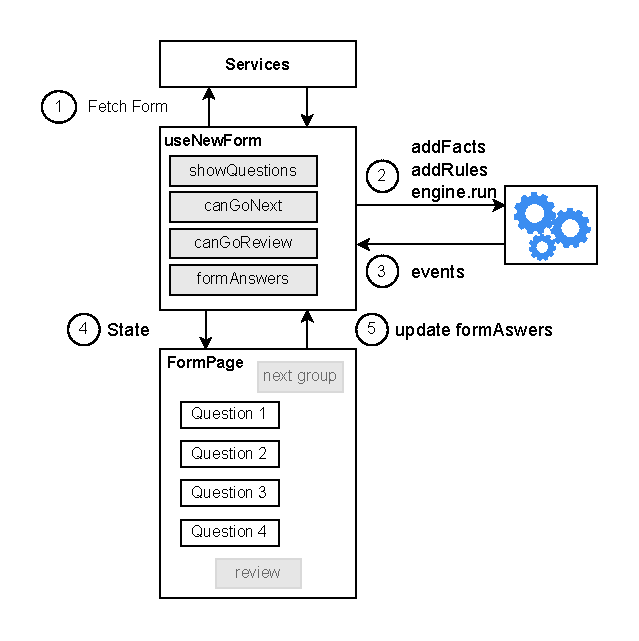
\includegraphics{./figures/JRE_implementation.pdf}}
	\end{center}
	\caption{Form implementation.}\label{fig:form_implementation}
\end{figure}

\newpage

\subsection{EditFormPage \& useEditFormPage}
The EditFormPage component acts a an outlet for the backoffice component page. It leverages the useEditFormPage hook to retrieve the form structure from the backend and manage it's state.

As mentioned in Section \ref{arc_jre}, the type of form events in our system are:
\begin{itemize}
	\item \textbf{showQuestion:} show the question with id in the params field;
	\item \textbf{nextGroup:} allow for navigation to next group, is triggered when all the question in current group have been answered;
	\item \textbf{showReview:} allow form review, is triggered when all the answers in the form have been answered and donor can review form.
\end{itemize}

To generate the nextGroup event we iterate over all the group of questions and for each create a top level condition of the all type and then iterate over every question in that group to create more conditions within this top level condition.
These questions can be divided into two types, which generate different conditions:
\begin{itemize}
	\item \textbf{Independent questions:} These generate the simplest conditions, since they just need to have an answer;
	\item \textbf{Child questions:} If the question is a child of another question there are two possible scenarios, either the question is visible and it needs an answer or it isn't displayed and should be ignored. 
\end{itemize}

The first scenario generates a condition as illustrated in Listing \ref{independent_questions}.
\begin{lstlisting}[style=sharpc, caption={Condition generated by and independent questions}, label={independent_questions}]
conditions: {
	all: [
		{
			fact: 'IndependentQuestion1',
			operator: 'notEqual',
			value: ''
		},
		{
			fact: 'IndependentQuestion2',
			operator: 'notEqual',
			value: ''
		}
	],
}
\end{lstlisting}

Meanwhile the second scenario generates a condition as illustrated in Listing \ref, the all top level condition type is used as a question can have multiple parent questions.

\begin{lstlisting}[style=sharpc, caption={Condition generated by and independent questions}, label={independent_questions}]
	conditions: {
		all: [
			any: [
				{
					fact: 'ChildQuestion',
					operator: 'notEqual',
					value: ''
				},
				all:{
					fact: 'ParentQuestion',
					operator: 'notEqual',
					value: 'value that trigger child question display'
				}
			]
		],
	}
\end{lstlisting}


As the user edit's the form's structure the changes are reflected in the hook's state, which is specially difficult given that a question can be a parent, i.e. it's answer causes another question to appear, and a child, i.e. it appears as a result of another question's answer.

To solve this issue the hook can reassign questions upon deletion, by finding the group with the parent question and setting the show condition of it's child question as undefined, which means they're automatically shown.

\subsection{EditTermsPage}

The EditTermsPage component acts as an outlet for the backoffice component page. It provides an interface for editing the terms and conditions. This component leverages the Editor component, which integrates the Jodit WYSIWYG editor, offering a rich text editing experience. The state management is handled using the useEditTerms custom hook, which ensures seamless interaction with the backend.
The content of the editor is stored as HTML allowing for flexible presentation and formatting when displayed to end-users.


\newpage

\section{Navigation}

This chapter features a navigation graph, presented in Figure ~\ref{fig:userNavigation}, that describes the UI flow of our platform.
The primary entry point for all users is the Home page, from which navigation diverges based on the user's login status and role.
With admins being able to navigate throughout the platform, while doctors lack backoffice access and finally donors only having access to the terms and form page.

\begin{figure}[H]
	\begin{center}
		\resizebox{150mm}{!}{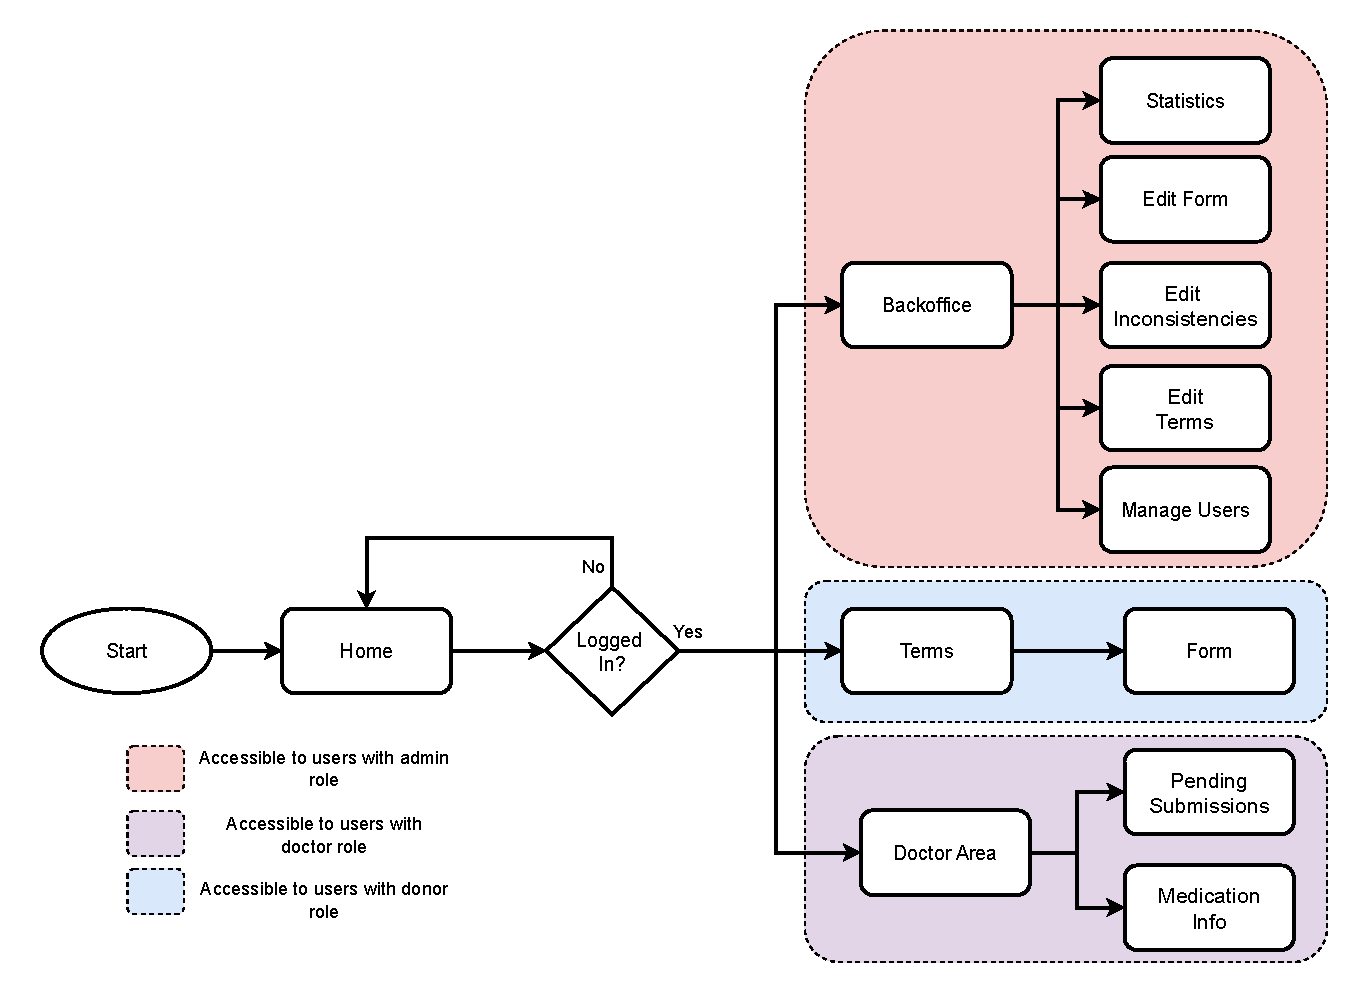
\includegraphics{./figures/userNavigation.pdf}}
	\end{center}
	\caption{UI navigation.}\label{fig:userNavigation}
\end{figure}

\section{Testing}
TO-DO










